% !TEX root =  reply_letter.tex
\clearpage
\section*{Response to 2nd Referee's Comments}
We would like to thank the Referee for their constructive comments, which have allowed us to considerably improve our paper. The main differences of the new version of the manuscript compared to the previous one can be found in the Discussion section.

You may find below our responses to the specific issues raised.

\begin{enumerate}
    \item \underline{Impact of increased use of MRIs on our risk calculator}

    We agree with the Referee that this is an important issue. In the recent years the use of MRIs to decide biopsies has increased. However, currently MRI data is extremely sparsely available in the PRIAS dataset. Hence, it may not be useful to include it in our model. However, in the next few years we expect to have enough MRI data, such as volume of the prostate tumor in the PRIAS dataset. This data can then be used as a third biomarker in our model, alongside PSA (prostate-specific antigen) and DRE (digital rectal examination) measurements. We expect that this extended model will lead to better risk predictions than using information from MRIs alone. 

    The current model (without MRI data) can also be used to decide the time of conducting an MRI. This is especially relevant for patients in developing countries, where an MRI scan is still expensive.

    We have added the aforementioned points briefly in the discussion section of the manuscript.

    \item \underline{Use of patient characteristics, and quality of life in the simulation}

    We agree with the Referee that this is an important issue. Currently, the model fitted to the PRIAS dataset, which is also used as the simulation model, accounts for patient age. The Referee also noted the importance of other factors such as having a first degree relative with cancer. However, this factor has been found to be predictive of cancer progression only in African-American patients \citep{telang2017prostate,goh2013clinical}. This is also evident by the fact that PRIAS and many other surveillance programs do not utilize this information in their biopsy protocols \citep{bokhorst2016decade,nieboer2018active}. In addition, patients who have a higher risk of an aggressive form of cancer are usually not recommended active surveillance. Hence the proposed model is relevant only for low-risk prostate cancer patients eligible for active surveillance. An exception are the active surveillance patients who are old and/or have comorbid illnesses. Currently, such patients may be removed from active surveillance and are instead offered the less intensive watchful waiting \citep{bokhorst2016decade} option. While it is possible to model watchful waiting as a competing risk in our model, but this falls outside the scope of the current work. 

    \textbf{How the findings of the model should be utilized in the larger clinical context and what additional work will be needed before the model can be used clinically?}
    The use of our model and the proposed approach in practice requires further work. A first step will be to initiate studies to look at feasibility acceptability and usability of the personalized approach in daily clinical practice. Biopsy decision making may include other factors such quality of life, patient preferences etc., which are not included in this model. However having an objective estimate (cancer progression risk) next to patient and care giver considerations (subjective) will aid shared decision making. To facilitate such shared decision making we have developed a web-application for clinicians (see Figure \ref{fig:webapp2}). We expect to hand it over to clinicians after an external validation of our model in active surveillance cohorts similar to PRIAS. This latter work is currently under progress.

    \begin{figure}[!htb]
	    		\centerline{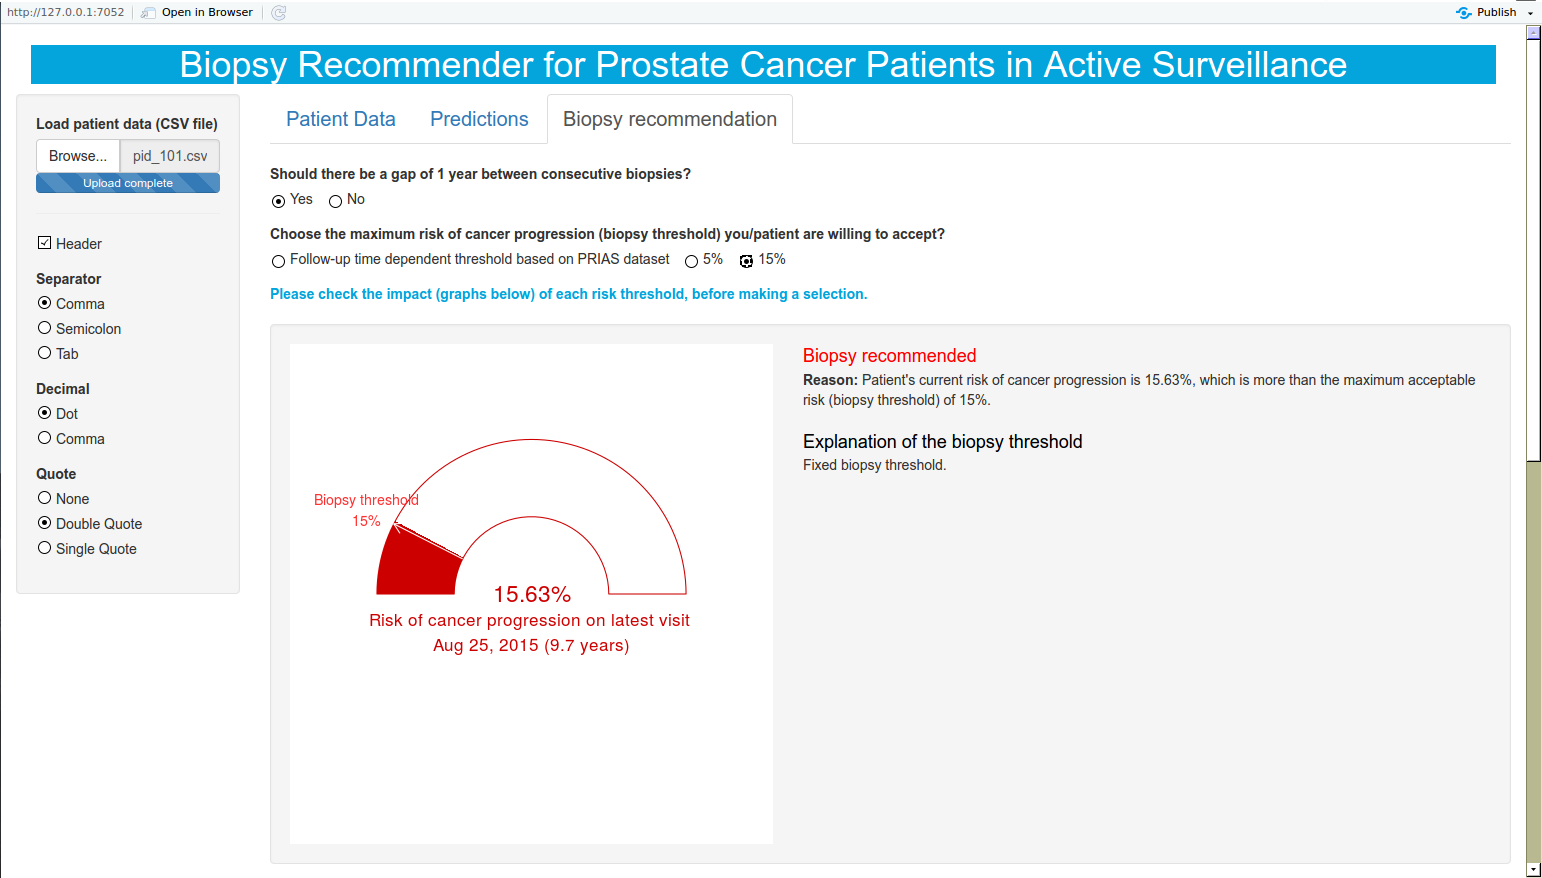
\includegraphics[width=0.8\columnwidth]{../images/webapp.png}}
				\caption{Web-based risk calculator for prediction of risk of prostate cancer progression.}
				\label{fig:webapp2}
			\end{figure}
    
\end{enumerate}

